%! Author = jiang-ziyang
%! Date = 22-7-4

% Preamble
\documentclass{ctexart}

% Packages
\usepackage{graphicx}
\usepackage{float}
\usepackage{subfigure}
\usepackage{amsmath}
\usepackage{amsfonts}
\usepackage{amsthm}
\usepackage{xcolor}
\usepackage[backref]{hyperref}
\usepackage{cite}
\usepackage{stmaryrd}
\usepackage{epstopdf}
\usepackage{tikz}
\usepackage{ctex}
\usepackage{amssymb}
\usepackage{wasysym}
\usetikzlibrary{shapes,positioning}
\usepackage{listings}
\tikzstyle{inout}=  [draw,
trapezium,
trapezium left angle = 65,
trapezium right angle = 115,
trapezium stretches,
] %%输入输出框
\tikzstyle{endn}=   [draw,
rounded rectangle,
]   %%起止框
\tikzstyle{exec}=   [draw,
rectangle,]    %%执行框 execute
\tikzstyle{judge}= [draw,
diamond,
inner sep=0,]   %%判断框
\lstset{
    basicstyle          =   \sffamily,          % 基本代码风格
    keywordstyle        =   \bfseries,          % 关键字风格
    commentstyle        =   \rmfamily\itshape,  % 注释的风格,斜体
    stringstyle         =   \ttfamily,  % 字符串风格
    flexiblecolumns,
    breaklines          =   true, %对过长的代码自动换行
    numbers             =   left,   % 行号的位置在左边
    showspaces          =   false,  % 是否显示空格,显示了有点乱,所以不现实了
    numberstyle         =   \zihao{-5}\ttfamily,    % 行号的样式,小五号,tt等宽字体
    showstringspaces    =   false,
    captionpos          =   t,      % 这段代码的名字所呈现的位置,t指的是top上面
    frame               =   lrtb,   % 显示边框
}



\title{一元二次方程在实数域上的求解}

\author{杨泽加 \\ 统计学 3190104662}

% Document
\begin{document}
    \bibliographystyle{IEEEtran}
    \maketitle

    \begin{abstract}
        本文介绍了一维非线性方程求根的算法实现和技术要点,并结合了数值算例及相关分析。
        旨在清晰地为读者提供一个理解该算法的角度。
    \end{abstract}


    \section{引言}\label{S1}
    对一维非线性方程的求根,算法库 gsl \cite{GSLhandwriting}为我们提供了二分法、牛顿法及 Steffenson 加速收敛法。
    本文将结合二分法和牛顿法展开讨论。 \\
    由于所有一维非线性方程    \\
    \begin{equation}
        \label{E1}
        f(x) = b, b \in \mathbb{C} \Rightarrow g(x) = f(x) - b = 0
    \end{equation}
    也是一个一维非线性方程,所以一维非线性方程的解总是可以转化为一维线性方程的求根问题。


    \section{数学理论}\label{S2}

    \subsection{二分法}\label{S2.1}
    对一个区间内单调的函数,若函数有实根,则函数曲线应当在根$x*$这一点上与
    x轴有一个交点,并且由于函数是单调的,在根附近的左右区间内,函数值的符号应当相反。
    利用这一特点,可以通过不断将求根区间二分的方法,每次将求根区间缩小为原来的一半,
    在新的折半后的区间内继续搜索方程的根,对根所在区间继续二分,直到求出方程的根为止。 \\
    这个算法的合理性由中值定理保证:\\
    \newtheorem{theorem}{定理}
    \begin{theorem}[中值定理]
        \label{T1}
        设函数 $f$ 在闭区间 $[a,b]$ 内连续且在开区间 $(a,b)$ 可微,则存在一点
        $c, a < c < b$,使得
        \begin{equation}
            \label{E2}
            f'(c) = \frac{f(b) - f(a)}{b - a}.
        \end{equation}
    \end{theorem}

    \subsection{牛顿法}\label{S2.2}

    牛顿法的基本思想是利用迭代点$x_k$处的一阶导数(梯度)和二阶导数(Hessen矩阵)
    对目标函数进行二次函数近似,然后把二次模型的极小点作为新的迭代点,并不断重复这一过程,
    直至求得满足精度的近似极小值。牛顿法的速度相当快,而且能高度逼近最优值。\\
    将 $f(x)$ 在 $x_0$ 点附近展开成 Taylor 级数\\
    \begin{equation}
        \label{E3}
        f(x) = f(x_0) + (x-x_0)f'(x_0) + (x-x_0)^2\frac{f''(x_0)}{2!} + \cdots
    \end{equation}
    取其线性部分作为非线性方程 $f(x) = 0$ 的近似方程,则有\\
    \begin{equation}
        \label{E4}
        f(x_0) + f'(x_0)(x-x_0) = 0
    \end{equation}
    设 $f'(x_0)\neq 0$,则其解为\\
    \begin{equation}
        \label{E5}
        x_1 = x_0 - \frac{f(x_0)}{f'(x_0)}
    \end{equation}
    如此得到了牛顿法的一个迭代序列
    \begin{equation}
        \label{E6}
        x_{n+1} = x_n - \frac{f(x_n)}{f'(x_n)}
    \end{equation}
    同时,为了避免牛顿法计算导数带来的开销,还可简化为:
    \begin{equation}
        \label{E7}
        \begin{aligned}
            x_{n+1} &= x_n - \frac{f(x_n)}{f'(x_0)}\\
            \text{or}\ x_{n+1} &= x_n - \frac{f(x_n)}{f(x_n) - f(x_{n-1})}(x_n-x_{x-1}\text{(差商代替导数)}
        \end{aligned}
    \end{equation}


    \section{算法介绍}\label{S3}

    \subsection{二分法}\label{S3.1}
    \begin{tikzpicture}[font=\small, scale=0.05]
        \node[endn] (start) {开始};
        \node[inout, below=0.5cmof start] (input) { 找出并输入根的存在区间$(a,b)$、精确度$\varepsilon$和最大迭代次数$M$};
        \node[exec, below=0.5cm of input] (init) {$k=0$};
        \node[judge, below=0.5cm of init] (interval_judge) {$b-a\geqslant\varepsilon$};
        \node[exec, below=0.5cm of interval_judge] (calc_mid) {$mid = \frac{b-a}{2}$};
        \node[judge, below=0.5cm of calc_mid] (judge_mid) {$f(a)f(mid)>0$};
        \node[exec,below left =of judge_mid] (set_a) {$a = mid$};
        \node[exec, below right=of judge_mid] (set_b) {$b = mid$};
        \node[exec, below = 2cm of judge_mid] (set_k) {$k = k + 1$};
        \node[judge, below=0.5cm of set_k] (judge_k) {$k \geqslant M$};
        \node[draw=none, right=3cm of judge_k] (middle) {};
        \node[exec, below=0.5cm of judge_k] (judge_k_deny_output) {超过最大迭代次数,迭代失败,迭代区间为$[a,b]$};
        \node[exec, left=0.5cm of judge_k_deny_output] (result) {输出$result = \frac{a+b}{2}$};
        \node[endn, below=0.5cm of judge_k_deny_output] (end) {结束};

        \draw[-latex] (start) edge (input) (input) edge (init) (init) edge (interval_judge);
        \draw[-latex] (interval_judge) edge node[pos=0.25,fill=white,inner sep=2pt]{Yes} (calc_mid)
        (interval_judge) -| node[pos=0.25,fill=white,inner sep=2pt]{No} (result);
        \draw[-latex] (calc_mid) edge (judge_mid);
        \draw[-latex] (judge_mid) -| node[pos=0.25,fill=white,inner sep=2pt]{Yes} (set_a);
        \draw[-latex] (judge_mid) -| node[pos=0.25,fill=white,inner sep=2pt]{No} (set_b);
        \draw[-latex] (set_a) |- (set_k);
        \draw[-latex] (set_b) |- (set_k);
        \draw[-latex] (set_k) edge (judge_k);
        \draw[-latex] (judge_k) edge node[pos=0.25,fill=white,inner sep=2pt]{Yes} (judge_k_deny_output);
        \draw (judge_k) edge  (middle);
        \draw[-latex] (middle) |- node[pos=0.25,fill=white,inner sep=2pt]{No} (interval_judge);
        \draw[-latex] (judge_k_deny_output) edge (end)
        (result) |- (end);
    \end{tikzpicture}

    \subsection{牛顿法}\label{S3.2}
    \begin{tikzpicture}[font=\small,thick, scale=0.1]
        \node[endn] (start) {开始};
        \node[inout, below=0.5cm of start] (input) {输入$x_0$和精度$\varepsilon$};
        \node[judge, below=0.5cm of input] (judge1) {$f'(x_0) = 0$};
        \node[exec,right =of judge1] (fail) {失败};
        \node[exec, below=0.5cm of judge1] (item) {$x_1=x_0 - \frac{f(x_0)}{f'(x_0)}$};
        \node[judge, below=0.5cm of item] (judge2) {$|x_1-x_0|<\varepsilon$};
        \node[exec, left=of item] (set_x) {$x_0 = x_1$};
        \node[inout, below=0.5cm of judge2] (output) {输出$x$};
        \node[endn, below=0.5cm of output] (end) {结束};

        \draw[-latex] (start) edge (input) (input) edge (judge1);
        \draw[-latex] (judge1) edge node[pos=0.25,fill=white,inner sep=2pt]{Yes} (fail)
        (judge1) edge node[pos=0.25,fill=white,inner sep=2pt]{No} (item);
        \draw[-latex] (fail) |- (end);
        \draw[-latex] (item) edge (judge2)
        (judge2) edge node[pos=0.25,fill=white,inner sep=2pt]{Yes} (output)
        (output) edge (end);
        \draw[-latex] (judge2) -| node[pos=0.25,fill=white,inner sep=2pt]{No} (set_x);
        \draw[-latex] (set_x) |- (judge1);
    \end{tikzpicture}


    \section{算法收敛性的比较}\label{S4}
    比较两种方法对1——10000的数字的求平方根结果如下:
    \begin{lstlisting}
10000次二分法迭代用时为850毫秒
10000次牛顿法迭代用时为1662毫秒
    \end{lstlisting}
    迭代次数的差异如下:
    \begin{figure}[H]
        \centering
        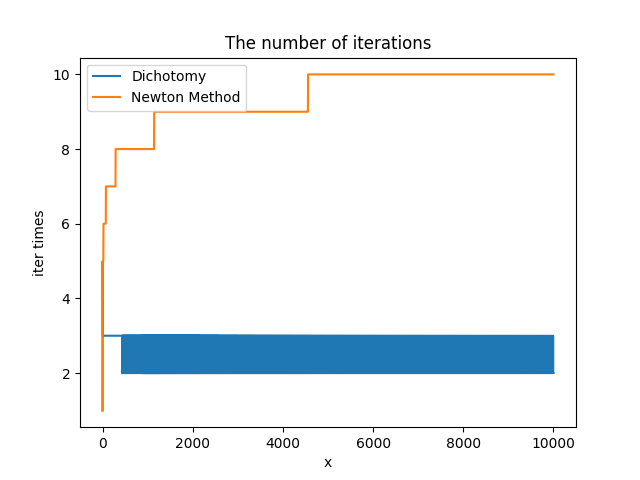
\includegraphics{./src/item}
    \end{figure}
    由于我迭代的起始区间均为迭代区域的最大值 $\max(a,b)$。牛顿法对初值较为敏感,故迭代次数较多。
    而在起初区间较小时,牛顿法的效果则好于二分法。\\
    因此我们在根的估计区间较小时使用牛顿法,否则建议使用二分法。
    \bibliography{reference}
\end{document}